\section{MOTIVATING EXAMPLE}
\label{sec:motivate}
\afterpage{
\begin{figure*}[!ht]
    \centering
    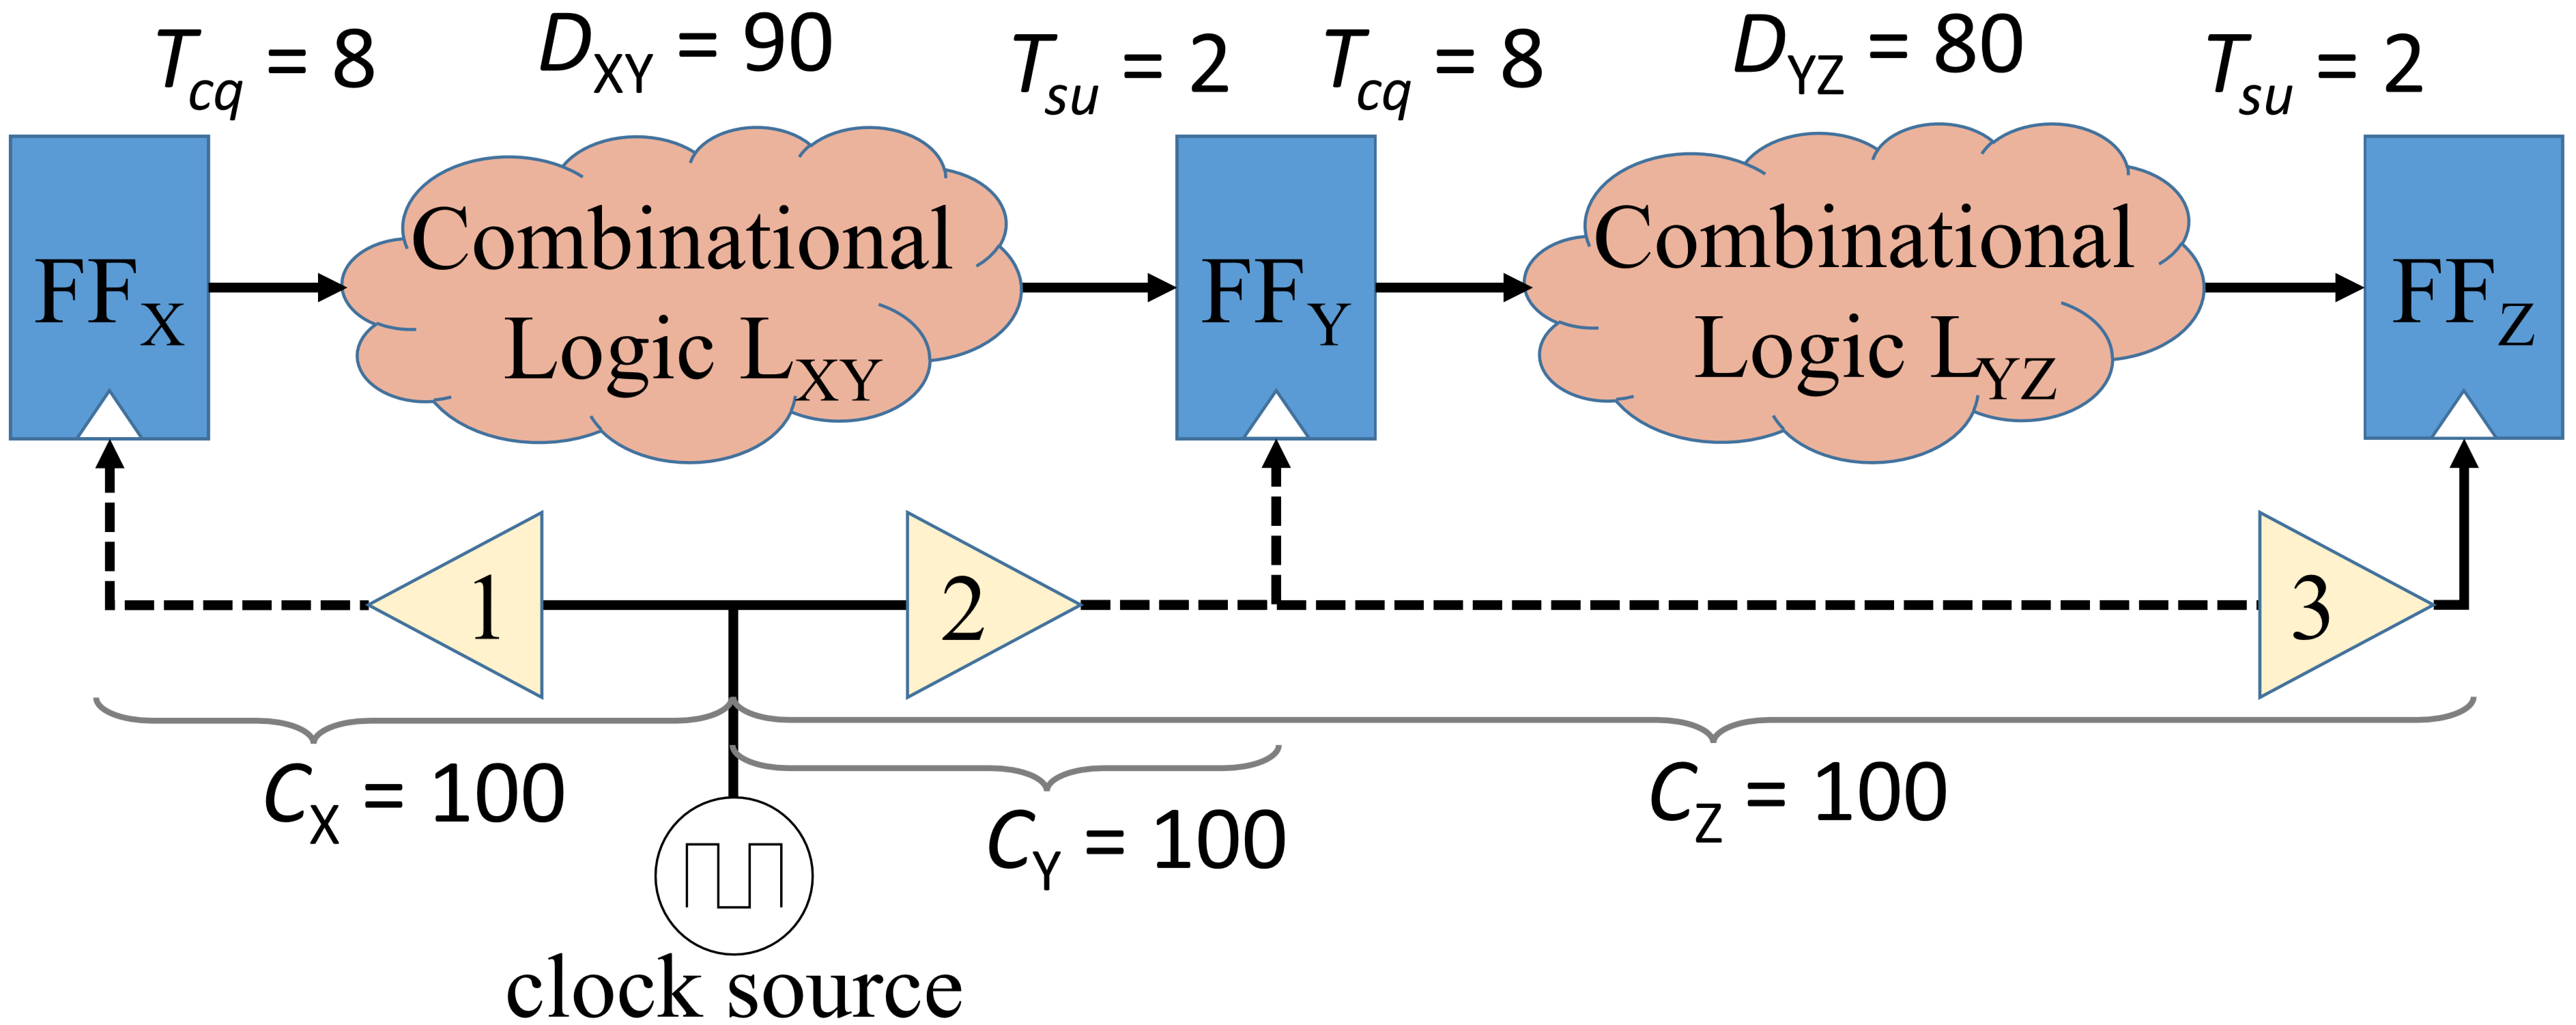
\includegraphics[width=0.9\columnwidth]{Motivating_example.png} 
    \caption{Illustrative example for the proposed framework based on DCC deployment and $V_{th}$ assignment}
    \label{fig:sub:example}
\end{figure*}

\begin{figure*}[!ht]
    \centering
    \label{fig:sub:notations}
    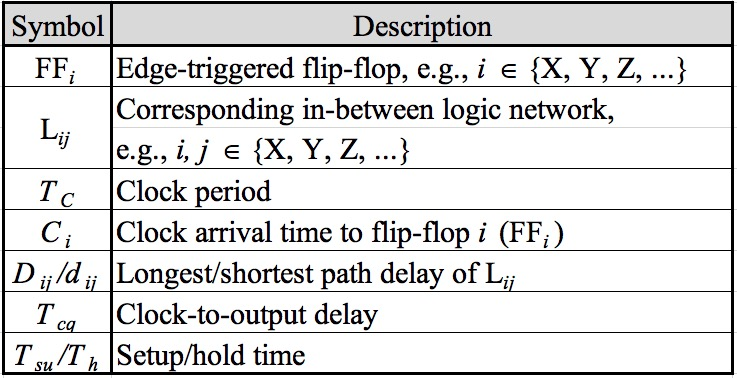
\includegraphics[width=0.6\columnwidth]{Notations.png} 
    \caption{Notations used in the paper}
    \label{fig:sub:notations}
\end{figure*}
}

This section introduces the example of motivating our idea of making aging useful. In Section~\ref{sec:mot:exp1}, we explore and recycle the useful aging-induced clock skew by manipulating the aging rates of clock paths. In Section~\ref{sec:mot:exp2}, high-$V_{th}$ assignment for clock buffers is incorporated to further enhance the benefit of aging-induced clock skews for aging tolerance. 

\subsection{Manipulating Aging Rates of Clock Paths}
\label{sec:mot:exp1}
Consider the circuit in Figure~\ref{fig:sub:example} where \ce{FF_X}, \ce{FF_Y} and \ce{FF_Z} are three edge-triggered flip-flops, and \ce{L_{XY}} and \ce{L_{YZ}} are the corresponding in-between logic networks. Other notations to be used later are listed in Figure~\ref{fig:sub:notations}.

For each pair of flip-flops (e.g., \ce{FF_i} and \ce{FF_j}) between which there exists at least one logic path from \ce{FF_i} to \ce{FF_j}, the following setup-time (Equation (\ref{eq:tsu})) and hold-time (Equation (\ref{eq:th})) constraints need to be satisfied:
\begin{equation}
	\fontsize{9}{9.6} C_i+T_{cq}+D_{ij}+T_{su}<C_j+T_c
	\label{eq:tsu}
\end{equation}
\begin{equation}
	\fontsize{9}{9.6} C_i+T_{cq}+d_{ij}<C_j+T_h
	\label{eq:th}
\end{equation}

Assume that, at year 10, $D_{ij}$ is degraded by 15\%, and both $T_{cq}$ and $T_{su}$ increase by 20\%. By using the predictive model presented in~\cite{wang2010impact, wang2007efficient, amrouch2016reliability}, we can accurately derive the aging of $C_i$ and $C_j$ due to the regularity and predictability of a typical clock waveform of 50\% duty cycle. In the process technology used (TSMC 45nm GP standard cell series), $C_i$ and $C_j$ are degraded by 13\% under 10-year BTI, i.e., $C_i$ and $C_j$ become 1.13X larger.

To be aging-aware for the example circuit in Figure~\ref{fig:sub:example}, we have to consider aforementioned aging factors in the setup-time constraints on \ce{L_{XY}} and \ce{L_{YZ}}:
\begin{equation}
	\fontsize{9}{9.6}\selectfont \ce{L_{XY}}:\quad \textbf{1.13}C_X+1.2T_{cq}+1.15D_{XY}+1.2T_{su}<\textbf{1.13}C_Y+T_c
\label{eq:lxy}
\end{equation}
\begin{equation}
	\fontsize{9}{9.6}\selectfont \ce{L_{YZ}}:\quad\textbf{1.13}C_Y+1.2T_{cq}+1.15D_{YZ}+1.2T_{su}<\textbf{1.13}C_Z+T_c
\label{eq:lyz}
\end{equation}
where $C_X$ = $C_Y$ = $C_Z$ = 100, $T_{cq}$ = 8, $T_{su}$ = 2, $D_{XY}$ = 90 and $D_{YZ}$ = 80, as shown in Figure~\ref{fig:sub:example}.
\begin{flushleft}
	By re-arranging Equations (\ref{eq:lxy}) and (\ref{eq:lyz}):
	{\fontsize{9}{9.6}
	\begin{flalign*}
		\hspace{0.6em}\ce{L_{XY}}: T_c &> 115.5 &\\
		\hspace{0.6em}\ce{L_{YZ}}: T_c &> 104
	\end{flalign*}
	}
\end {flushleft}
Therefore, the clock period needs to be larger than 115.5 (dominated by \ce{L_{XY}}) to ensure no setup-time violation over a required lifespan of 10 years. For brevity, we omit the discussion on hold-time constraints, which in our work are actually formulated to ensure no existence of racing due to short paths.

For the objective of minimizing required $T_c$ under aging, we insert one 20\% \textit{duty-cycle converter} (DCC) at the input of buffer 1, and another 80\% DCC at the input of buffer 2. The 20\% (80\%) DCC can decrease (increase) the stress times of downstream clock buffers by converting the clock duty cycle to 20\% (80\%), from a typical duty cycle of 50\%. Therefore, 20\% DCC can mitigate/decelerate the aging of $C_X$ and 80\% DCC can aggravate/accelerate the aging of $C_Y$. In the case of no DCC, $C_X$ and $C_Y$ are degraded by 13\% under 10-year BTI in TSMC 45nm GP standard cell series, while 20\% and 80\% DCCs will degrade $C_X$ and $C_Y$ by 9\% and 16\%, respectively, assuming that the clock paths from the clock source to \ce{FF_X} and \ce{FF_Y} are disjoint.

Consider the new aging factors (due to effects of various clock duty cycles) in the setup-time constraints on \ce{L_{XY}} and \ce{L_{YZ}}:
\begin{equation}
	\fontsize{9}{9.6}\selectfont \ce{L_{XY}}:\quad \textbf{1.09}C_X+1.2T_{cq}+1.15D_{XY}+1.2T_{su}<\textbf{1.16}C_Y+T_c 
	\label{eq:lxy2}
\end{equation}
\begin{equation}
	\centering
	\fontsize{9}{9.6}\selectfont \ce{L_{YZ}}:\quad \textbf{1.16}C_Y+1.2T_{cq}+1.15D_{YZ}+1.2T_{su}<\textbf{1.16}C_Z+T_c
	\label{eq:lyz2}
\end{equation}
By re-arranging Equations (\ref{eq:lxy2}) and (\ref{eq:lyz2}):
{\fontsize{9}{9.6}
\begin{flalign*}
	\hspace{0.6em}\ce{L_{XY}}: T_c &> 108.5 &\\
	\hspace{0.6em}\ce{L_{YZ}}: T_c &> 104
\end{flalign*}
}
As it can be seen, we can reduce the required $T_c$ from 115.5 to 108.5 (dominated by \ce{L_{XY}} still), by adding two DCCs in the existing synthesized clock tree to create aging-induced clock skews. The skew for \ce{L_{XY}} (between \ce{FF_X} and \ce{FF_Y}), quantified as 1.16$C_Y$ minus 1.09$C_X$, is useful/beneficial and accounts for the reduction of required $T_c$. A certain level of aging tolerance is thus achieved because aging-induced performance degradation of $D_{XY}$ (plus $T_{cq}$ and $T_{su}$ actually) can be tolerated, by exploring such useful aging-induced clock skews.

\subsection{Assigning High-$V_{th}$ to Clock Buffers}
\label{sec:mot:exp2}
For the circuit in Figure~\ref{fig:sub:example}, the technique of high-$V_{th}$ assignment for clock buffers is incorporated to explore more beneficial clock skews and further reduce the required $T_c$. 

Given that a 20\%DCC and an 80\% DCC have been inserted at the inputs of buffers 1 and 2, respectively, we can alter buffer 2 and all its downstream buffers, by assigning them a higher threshold voltage, so as to achieve better utilization of clock skews. To include the timing information of high-$V_{th}$ buffers in the setup-time constraints, the fresh/intrinsic delay of a high-$V_{th}$ buffer is assumed to be 1.15X longer than that of a nominal-$V_{th}$ buffer, and aging rate of high-$V_{th}$ buffer, receiving a clock duty cycle of 80\%, is 8\%. %\cite{gomez2016early}\footnote{The aging rates of high-$V_{th}$ buffers are lower than those of nominal-$V_{th}$ buffers, because the higher/lower $V_{th}$ leads to lower/higher aging rate.}. 
Consider the new aging factors in the setup-time constraints on \ce{L_{XY}} and \ce{L_{YZ}}:
\begin{equation}
	\fontsize{9}{9.6}\selectfont \ce{L_{XY}}:\quad \textbf{1.09}C_X+1.2T_{cq}+1.15D_{XY}+1.2T_{su}<(\textbf{1.15} \times \textbf{1.08})C_Y+T_c
	\label{eq:lxy3}
\end{equation}
\begin{equation}
	\centering
	\fontsize{9}{9.6}\selectfont \ce{L_{YZ}}:\quad (\textbf{1.15} \times \textbf{1.08})C_Y+1.2T_{cq}+1.15D_{YZ}+1.2T_{su}<(\textbf{1.15} \times \textbf{1.08})C_Z+T_c
	\label{eq:lyz3}
\end{equation}
By re-arranging Equations (\ref{eq:lxy3}) and (\ref{eq:lyz3}):
{\fontsize{9}{9.6}
\begin{flalign*}
	\hspace{1.2em}\ce{L_{XY}}: T_c &> 100.3 &\\
	\hspace{1.2em}\ce{L_{YZ}}: T_c &> 104
\end{flalign*}
}
Apparently, the required $T_c$ can be further reduced/optimized from 108.5 to 104 (dominated by \ce{L_{YZ}} rather than \ce{L_{XY}} as in Section~\ref{sec:mot:exp1}), by inserting two DCCs and assigning a higher $V_{th}$ to certain buffers. As it can be seen, the skew for \ce{L_{XY}}, which equals $(1.15 \times 1.08)C_Y$ minus 1.09$C_X$, is larger than that in Section~\ref{sec:mot:exp1}. Therefore, the new skew for \ce{L_{XY}} is more useful/beneficial and accounts for better optimization of required $T_c$. 

%Note that, there exists a difference between DCC and high-$V_{th}$ buffer leader. DCC is a physical gate which is inserted at the inputs of certain clock buffers to manipulate the aging behaviors of downstream buffers. However, high-$V_{th}$ buffer leader is selected from existing clock buffers and indicates the start location where we begin assign high $V_{th}$ toward flip-flops. 

%Additionally, when it comes to the timing-borrowing mechanism of the two examples, there exists a difference: 1) The timing-borrowing mechanism, in the first example, is achieved by the aging-induced clock skew, caused by manipulating the duty-cycle delivered to flip-flops. 2) In the second example, the timing-borrowing mechanism is based on aging-induced clock skew and \textit{tech-induced} clock skew, which is caused by manipulating the technology of clock buffers, i.e., re-assign the $V_{th}$ of clock buffers. 

One may note that \textit{clock skew scheduling} (CSS)~\cite{fishburn1990clock}, which derives unequal delays for all clock branches prior to \textit{clock tree synthesis} (CTS), can also optimize a circuit for aging tolerance. However, the optimization potential of general CSS is limited since it is difficult to precisely implement a wide range of clock delays during CTS \cite{li2011optimal}. %In contrast, post-CTS clock skew scheduling based on buffer insertion is another option. We will demonstrate that, if buffer insertion is employed to match our optimization results based on DCC insertion, the number of inserted buffers is usually much larger than the number of inserted DCCs. Also, as described later in Section~\ref{subsec:tpc}, the overhead of a single DCC can be diminished by integrating a DCC with its downstream buffer, which further reveals the cost effectiveness of our proposed DCC-based framework.



